\documentclass[red]{beamer}

\usepackage{fixltx2e}

%\usetheme{MyTheme} 
%\usetheme{Berkeley}
\usetheme{Copenhagen}

% title
\title[Flocking Implementation for the Blender Game Engine]{Flocking Implementation for the Blender Game Engine}
\author{Myrna I. Merced Serrano}
\institute{\textbf{Adviser:} Dr. Gordon Erlebacher}
\date{June 24\textsuperscript{th}, 2011}

\setcounter{tocdepth}{1}

\begin{document}

%--------------------------------------------
% title 
%--------------------------------------------
\begin{frame}
	\titlepage
\end{frame}

%--------------------------------------------
% table of contents
%--------------------------------------------
\begin{frame}
	\tableofcontents
\end{frame}

%--------------------------------------------
% motivation - intro
%--------------------------------------------
\section{Motivation}

%--------------------------------------------
% educational games
%--------------------------------------------
\subsection{Educational Games}
\begin{frame}{Educational Games}
	\begin{itemize}
		\pause \item \textbf{Goal}: learn while you are playing
		\pause \item Some of the benefits of playing Educational Games are:
			\begin{itemize}
				\pause \item gain more knowledge
				\pause \item motivation
				\pause \item interest
			\end{itemize}
		\pause \item A game must be challenge, have fantasy and curiosity in order to be a fun Educational game.
	\end{itemize}	
\end{frame}
% ASK: HOW EDUCATIONAL GAMES OR ANY OTHER GAME CAN BE CREATED?
% ANSWER: USING GAME ENGINES

%--------------------------------------------
% GEs
%--------------------------------------------
\subsection{Game Engines}
\begin{frame}{Game Engines}
	\begin{itemize}
		\pause \item Game Engines (GE) are used to simulate partial reality.
		\pause \item Let you interact with 3D world in real-time. \pause FUN!
		\pause \item A GE consist of:
			\begin{itemize}
				\pause \item render the 3D world and the objects on it
				\pause \item rerender the world when something change
				\pause \item game logic
				\pause \item simulate the physics
				\pause \item collision detection and reaction
			\end{itemize}
	\end{itemize}
\end{frame}

%--------------------------------------------
% aim
%--------------------------------------------
\begin{frame}{Aim}
	\begin{itemize}
		\pause \item To develop a flocking implementation that can be used in the Blender Game Engine
	\end{itemize}
\end{frame}

%--------------------------------------------
% BGE
%--------------------------------------------
\begin{frame}{The Blender Game Engine}
	\begin{itemize}
		\pause \item BGE is a very powerful tool.
		\pause \item Games can be created without the need for explicit programming.
		\pause \item After creating the 3D scene you can bring it to life by using the simple logic editor.
			% figure: logic editor 
			\pause
			\begin{figure}[htbp]
			\begin{center}
			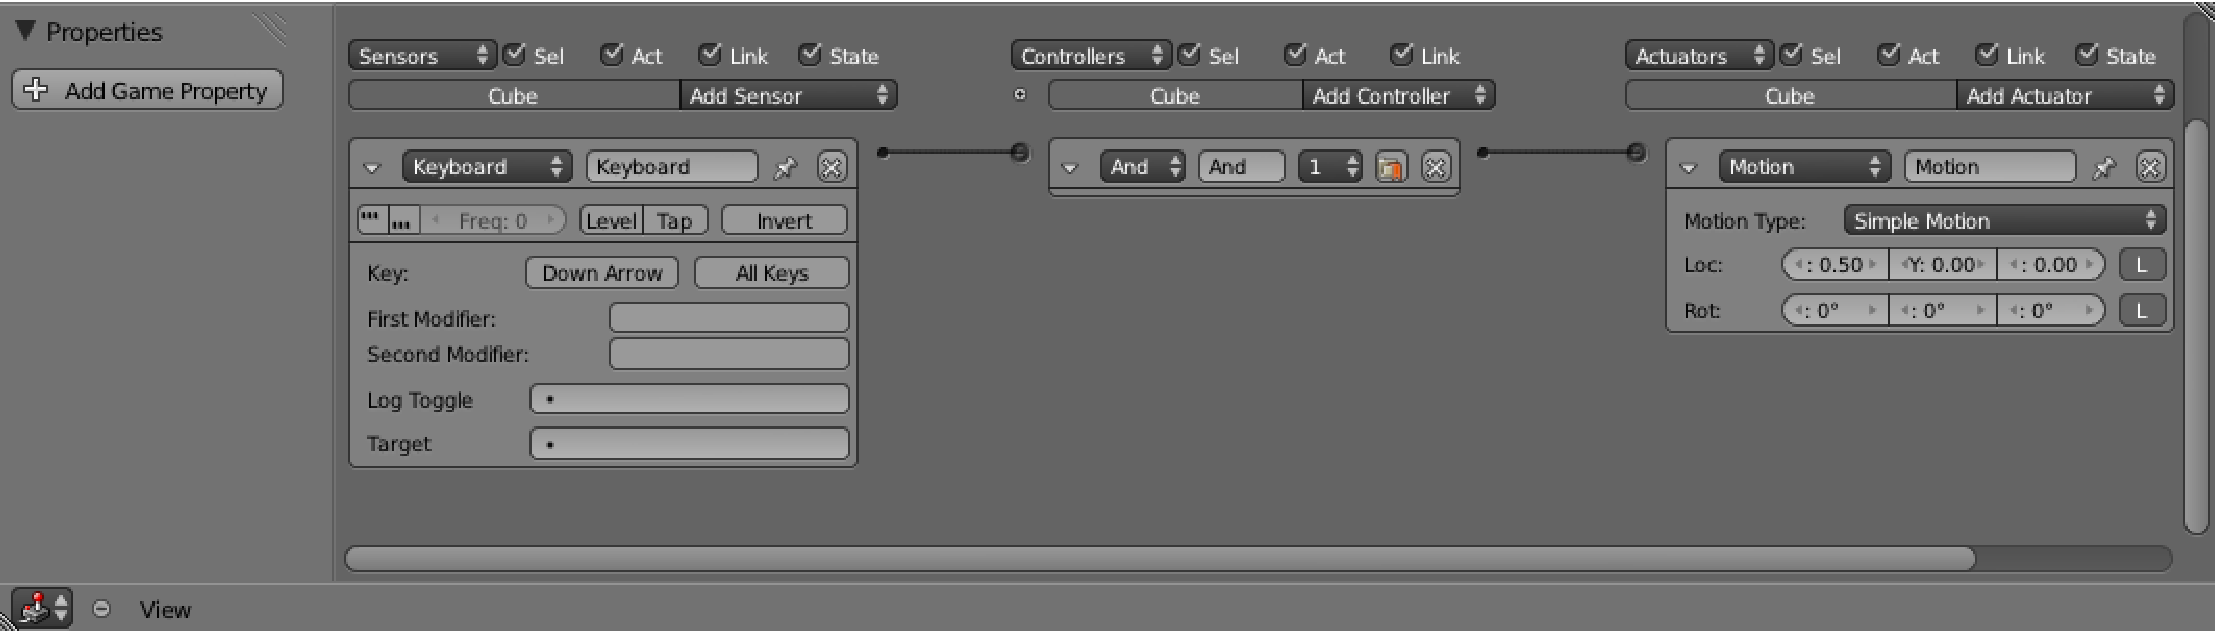
\includegraphics[scale=0.25]{../figures/logic.pdf}
			\caption{Blender Game Logic Editor}
			\label{logicEditor}
			\end{center}
			\end{figure}
	\end{itemize}
\end{frame}

%--------------------------------------------
% related work
%--------------------------------------------
\subsection{Background and Related Work}

\begin{frame}{Background and Related Work Outline}
	\begin{itemize}
		\pause \item Flocking
		\pause \item Early work
		\pause \item Current work
		\pause \item Applications
		\pause \item GPU computing
		\pause \item Flocking using the GPU
	\end{itemize}
\end{frame}

% flocking
\begin{frame}{Flocking}
	\begin{itemize}
		\pause \item \textit{Flocking} is a nature-inspired behavior, mostly seen in social animals.
		\pause \item Inspired by the behavior of birds Craig Reynolds developed a behavioral model that simulated the self-organization of \textit{boids}.
		\pause \item \textit{Boids} are the entities of a flock.
		\pause \item Since, Reynolds publication in 1987, the field of flocking became very popular and many applications have been published.
	\end{itemize}
\end{frame}

% craig
\begin{frame}{Original Boids Model by Craig Reynolds}
	\begin{itemize}
		\pause \item Craig Reynolds is the pioneer of flocking, his most recognized paper: \textit{Flocks, herds, and school: A Distributed Behavioral Model} revolutionized the field of flocking.
		\pause \item He stated that the behavior of the boids is represented by a set of rules and its internal state.
		\pause \item The set of rules, also called \textit{Boids Model}, that he defined consist of the following:
			\begin{itemize}
				\pause \item collision avoidance
				\pause \item velocity matching
				\pause \item flock centering
			\end{itemize}
	\end{itemize}
\end{frame}

% other rules
\begin{frame}{Proceeding Work}
	\begin{itemize}
		\pause \item In 1999 Reynolds expanded the set of behaviors.
		\pause \item Some of the new behaviors were:
			\begin{itemize}
				\pause \item seek and pursuit
				\pause \item flee and evasion
				\pause \item obstacle avoidance
				\pause \item path following
				\pause \item leader following
				\pause \item among others...
			\end{itemize}
	\end{itemize}
\end{frame}
		
% applications
\begin{frame}{Applications}
	\begin{itemize}
		\pause \item Prey and predator simulations
		\pause \item Crowding simulations
		\pause \item Robotics
		\pause \item Unmanned air vehicles
		\pause \item Document clustering
	\end{itemize}
\end{frame}

% GPU computing
\begin{frame}{GPU Computing}
	\begin{itemize}
		\pause \item \textit{GPU computing}, also know as \textit{GPGPU} is when we use GPUs for general computing.
		\pause \item \textit{GPU computing} is an heterogeneous system that uses GPUs and CPUs together to process a task.
		\pause \item GPUs are numeric computing engines.
		\pause \item GPUs have their own architecture therefore, they also have their own programming languages.
	\end{itemize}
\end{frame}

% flocking using the GPU
\begin{frame}{Flocking Using the GPU}
	\begin{itemize}
		\pause \item Flocking algorithms are parallelizable algorithms because the same operations are computed for all boids in the flock.
		\pause \item GPUs can be used to implement flocking algorithms and enhance the performance of the execution of the program.
	\end{itemize}
\end{frame}

%--------------------------------------------
% flocking algorithm
%--------------------------------------------
\section{Algorithm}

\begin{frame}{Flocking}
	\begin{itemize}
		\pause \item \textit{Flocking} is used to simulate social behavior between entities by following a simple set of rules.
		\pause \item These rules, also called \textit{steering behaviors} were introduced by Craig Reynolds and they are:
			\begin{itemize}
				\pause \item Separation
				\pause \item Alignment
				\pause \item Cohesion
			\end{itemize}
		\pause \item The steering behaviors are velocity vectors with direction and magnitude.
	\end{itemize}
\end{frame}

%--------------------------------------------
% 3 behaviors
%--------------------------------------------
\subsection{Three Main Steering Behaviors}

% separation
\begin{frame}{Separation}
	% equation: separation 
	\pause
	\begin{equation}
	\label{separationEquation}
	Separation =\frac{1}{M} \sum_{n=1}^{M} \frac{p_i - p_n}{d(p_i,p_n)}
	\end{equation}
	
	% figure: separation
	\pause
	\begin{figure}[htbp]
	\begin{center}
	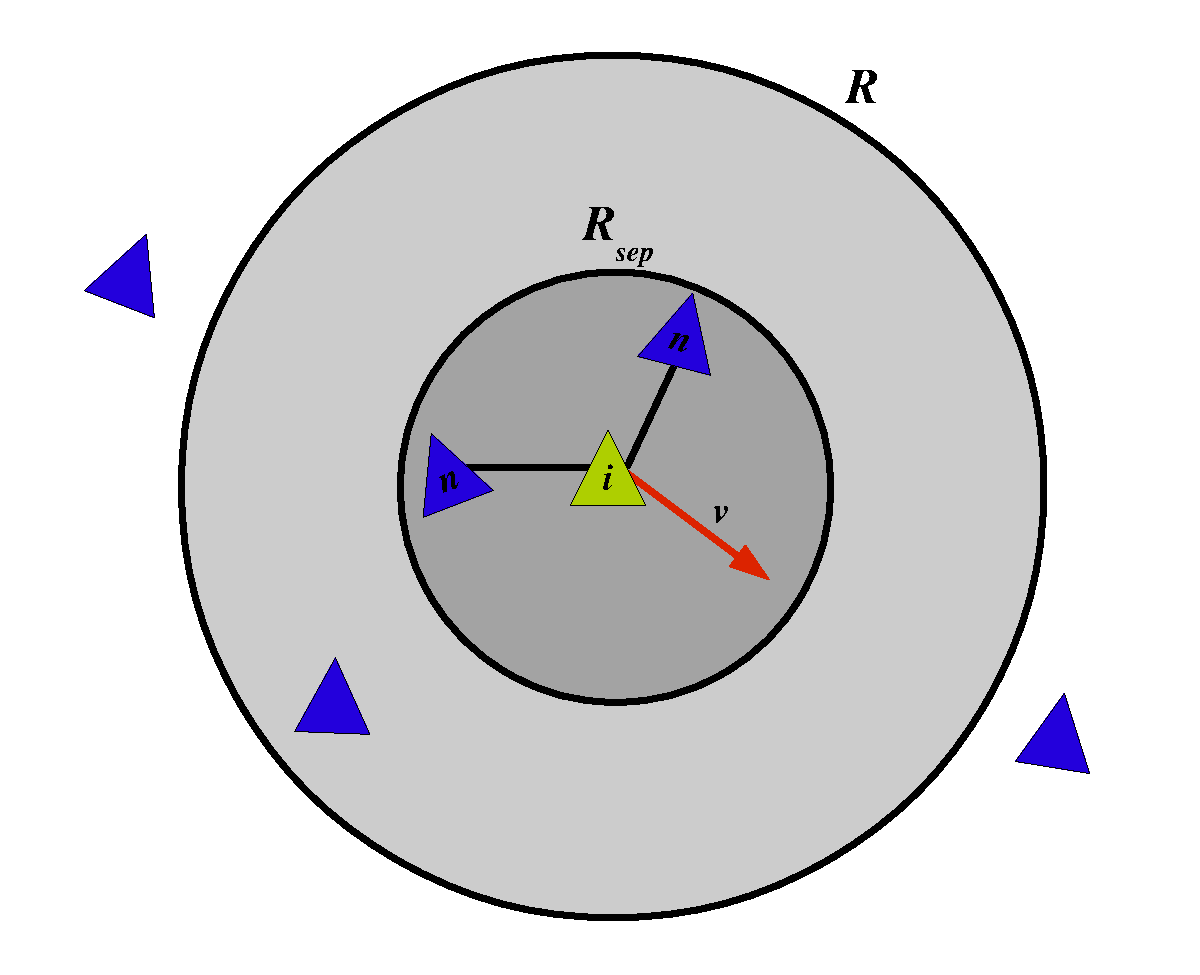
\includegraphics[scale=0.15]{../figures/separation.pdf}
	\caption{Separation steering behavior}
	\label{separation}
	\end{center}
	\end{figure}
\end{frame}

% alignment
\begin{frame}{Alignment}
	% equation: alignment
	\begin{equation}
	\label{alignmentEquation}
	Alignment = \left[  \frac{1}{N} \sum_{n=1}^{N} v_n \right ] - v_i
	\end{equation}
	
	% figure: alignment
	\pause
	\begin{figure}[htbp]
	\begin{center}
	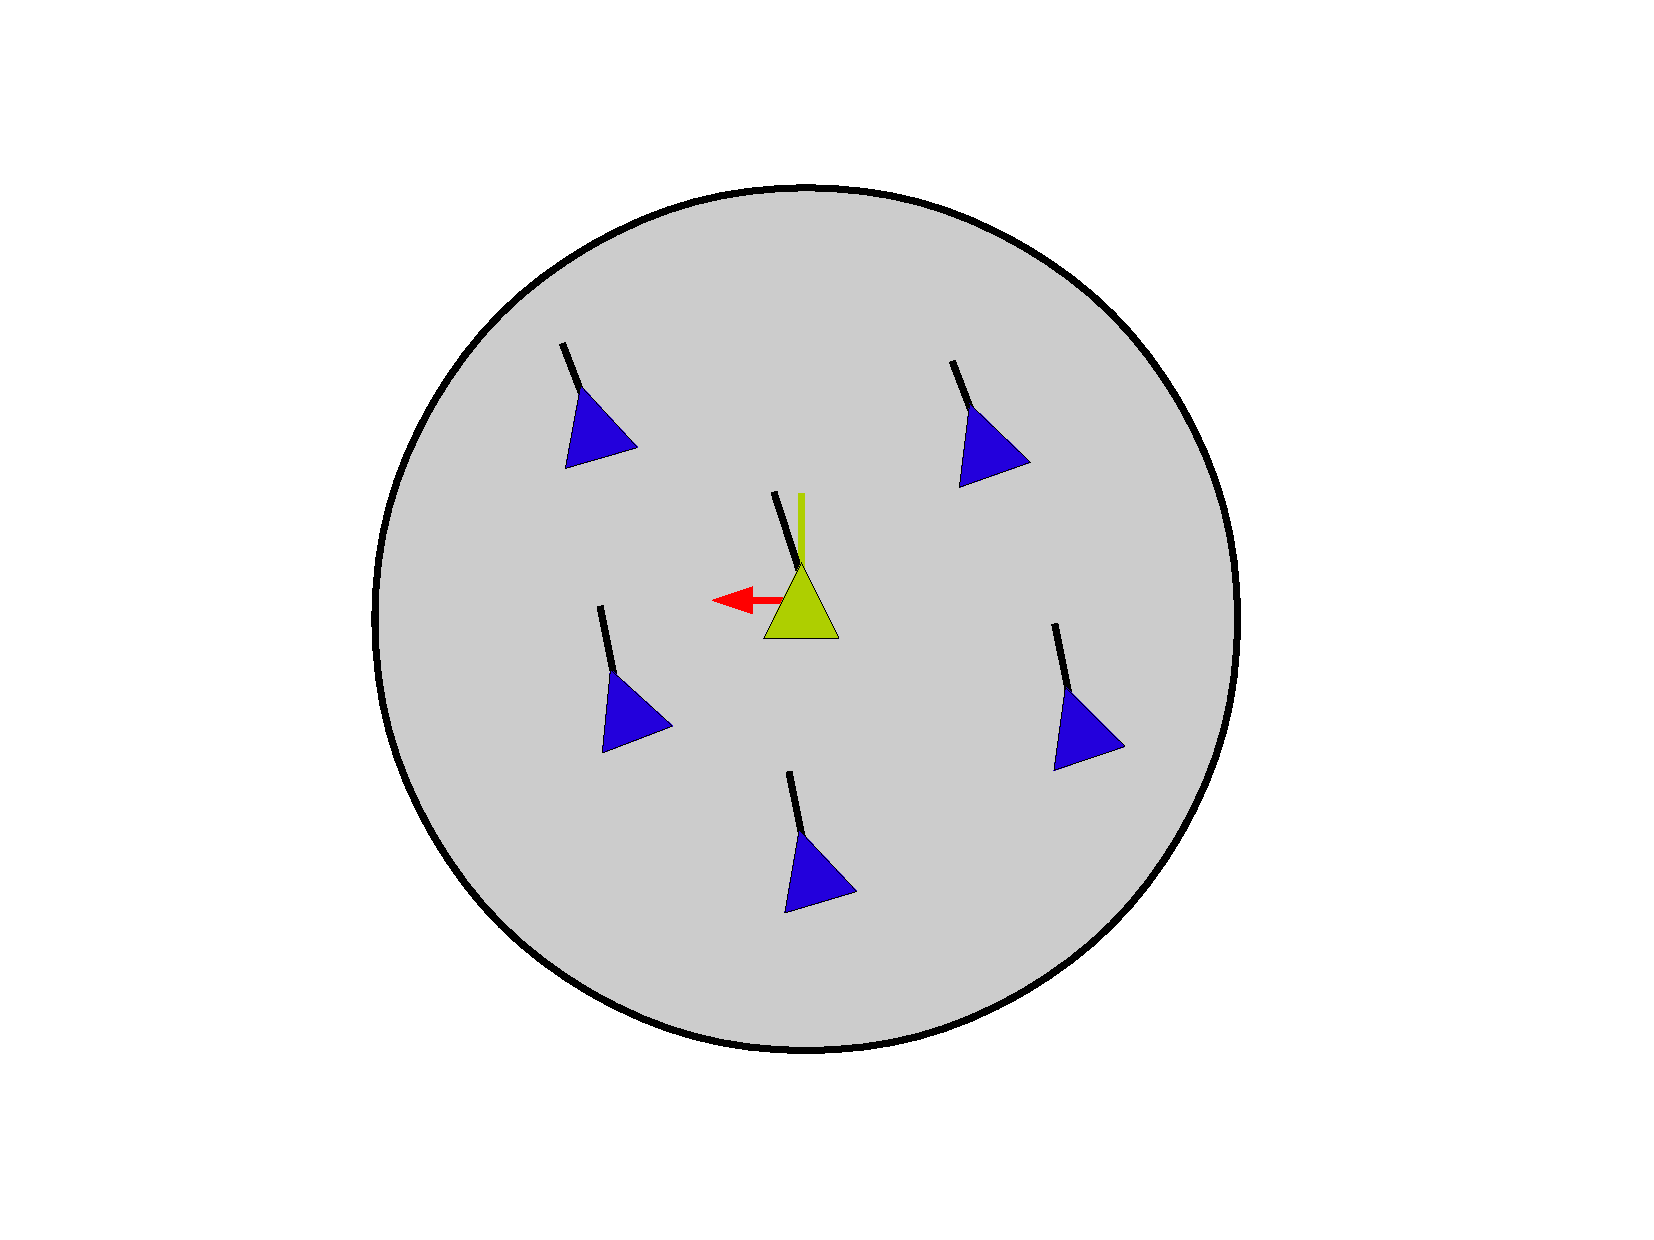
\includegraphics[scale=0.15]{../figures/alignment.pdf}
	\caption{Alignment steering behavior}
	\label{alignment}
	\end{center}
	\end{figure}
\end{frame}

% cohesion
\begin{frame}{Cohesion}
	% equation: cohesion
	\begin{equation}
	\label{cohesionEquation}
	Cohesion = \left[  \frac{1}{N} \sum_{n=1}^{N} p_n \right ] - p_i
	\end{equation}
	
	% figure: cohesion
	\pause
	\begin{figure}[htbp]
	\begin{center}
	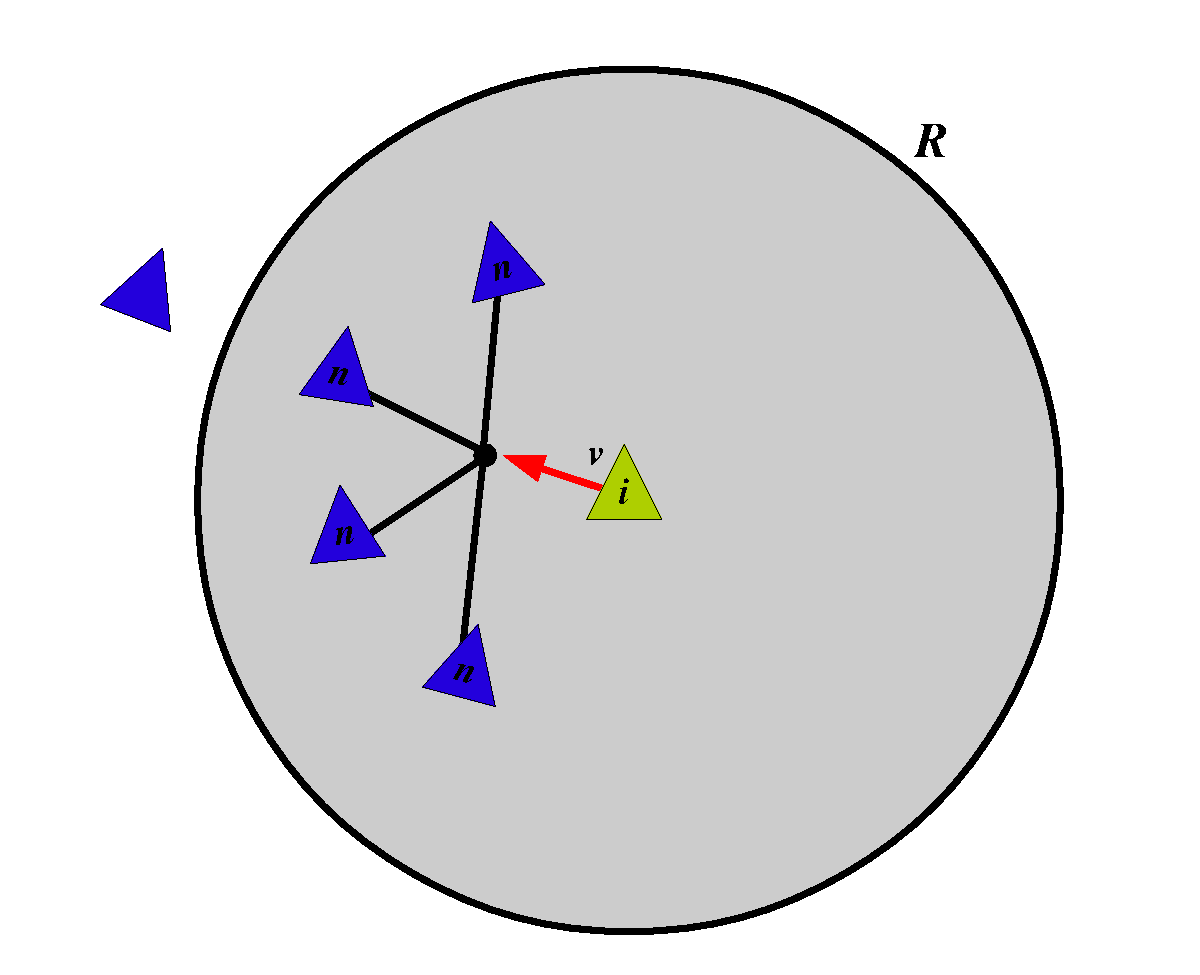
\includegraphics[scale=0.15]{../figures/cohesion.pdf}
	\caption{Cohesion steering behavior}
	\label{cohesion}
	\end{center}
	\end{figure}
\end{frame}

%--------------------------------------------
% other behaviors
%--------------------------------------------
\subsection{Other Steering Behaviors}

% goal and avoid
\begin{frame}{Goal and Avoid}
	% figure: seek and flee
	\pause
	\begin{figure}[htbp]
	\begin{center}
	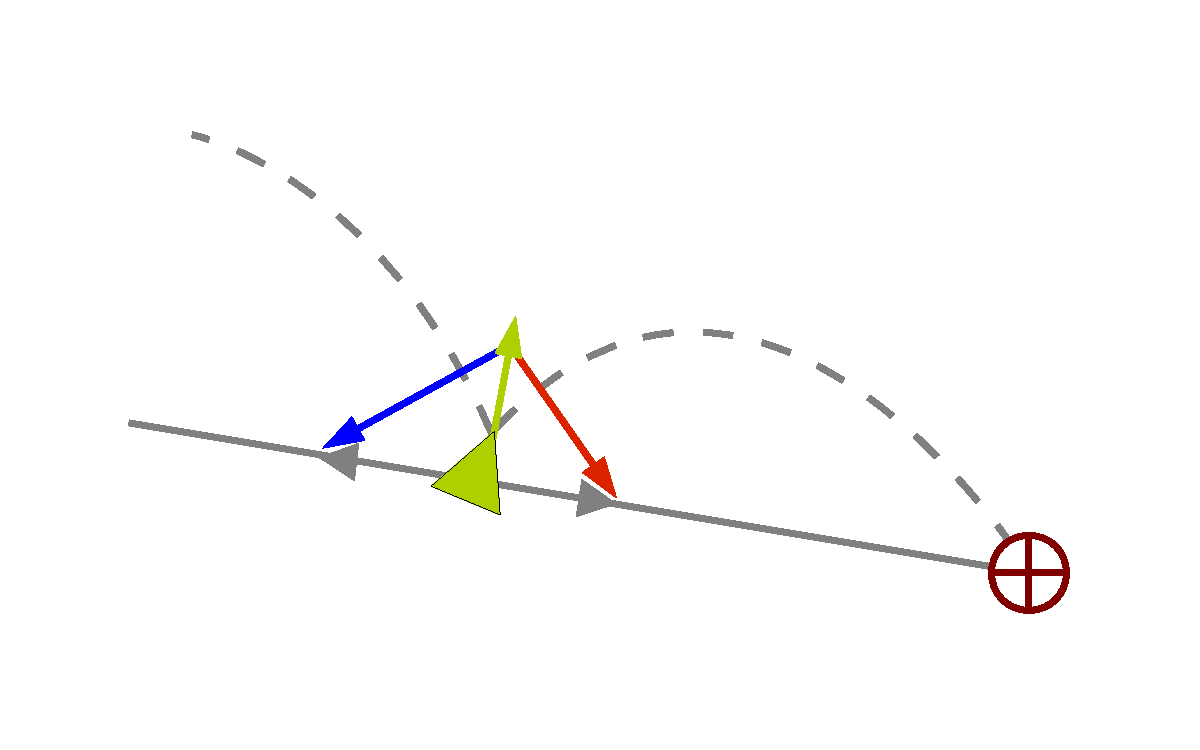
\includegraphics[scale=0.35]{../figures/seekANDflee.pdf}
	\caption{Goal and Avoid steering behavior}
	\label{seekANDflee}
	\end{center}
	\end{figure}
\end{frame}

% follow the leader
\begin{frame}{Follow the Leader}
	% figure: leader following
	\pause
	\begin{figure}[htbp]
	\begin{center}
	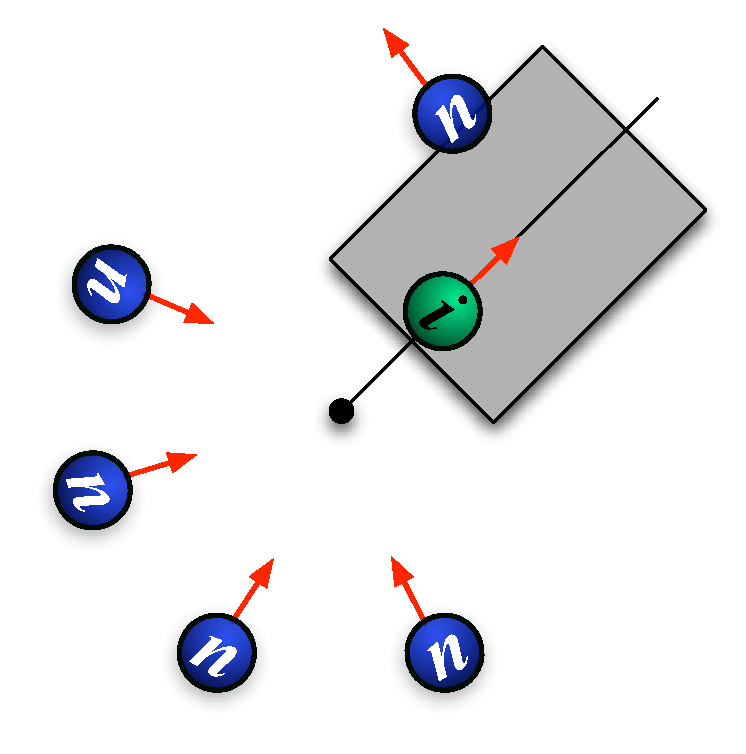
\includegraphics[scale=0.35]{../figures/leaderFollowing.pdf}
	\caption{Follow the leader steering behavior}
	\label{leadFollow}
	\end{center}
	\end{figure}
\end{frame}

%--------------------------------------------
% algorithm
%--------------------------------------------
\subsection{Flocking Algorithm}

% rules
\begin{frame}{Algorithm to compute the rules}
	\alert<1>{$for$ each neighbor $j$ of boid $i$ $do$}			\\
	\alert<2>{~~$if$ dist($i$, $j$) $<=$ searching radius $then$}	\\
	\alert<3>{~~~~flockmates++}							\\
	\alert<4>{~~$if$ $w_{sep}$ $>$ 0 $then$}					\\
	\alert<5>{~~~~$if$ dist($i$, $j$) $<=$ minimum distance $then$}	\\
	\alert<6>{~~~~~~nearestFlockmates++}						\\
	\alert<6>{~~~~~~s = $pos_i$ - $pos_j$} 					\\
	\alert<6>{~~~~~~s /= dist($i$, $j$)} 						\\
	\alert<6>{~~~~~~separation += s}							\\
	\alert<7>{~~$if$ $w_{align}$ $>$ 0 $then$}				\\
	\alert<7>{~~~~alignment += $vel_j$}						\\
	\alert<8>{~~$if$ $w_{coh}$ $>$ 0 $then$}					\\
	\alert<8>{~~~~cohesion += $pos_j$}						\\
\end{frame}

% integration
\begin{frame}{Combine and Integrate}
 	%\alert<1>{$acc_{sep}$ = separation * $w_{sep}$}			\\
	%\alert<1>{$acc_{align}$ = alignment * $w_{align}$}		\\
	%\alert<1>{$acc_{coh}$ = cohesion * $w_{coh}$}			\\ 
 	\alert<1>{Multiply each rule by its weight to get the respective acceleration.} 	\\
	%\alert<2>{$acc$ = $vel_i$ + $acc_{sep}$ + $acc_{align}$ + $acc_{coh}$} 	\\ 
	\alert<2>{Add the acceleration of each rule and the current velocity.} 	\\
	\alert<3>{Constraint the acceleration to a maximum speed.}			\\ 
	\alert<4>{Optional: Set any artificial velocity.}						\\ 
	%\alert<5>{$vel_i$ = $vel_{external}$ + $acc$}				\\ 
	\alert<5>{Add the artificial velocity to the acceleration to get the \textit{new} velocity.} \\
	%\alert<6>{$pos_i$ +=  $dt $* $vel_i$}					\\
	\alert<6>{Multiply the velocity by the time step.}			\\
	\alert<7>{Add the velocity to the position to get the \textit{new} position.}	\\
\end{frame}

% each frame
\begin{frame}{Algorithm to update the simulation at each frame}
%\begin{tabbing}
	%\begin{block}{Algorithm to update the simulation at each frame}
		\alert<1>{Create a FLOCK particle system.}	\\
		\alert<2>{$for$ each frame $do$}			\\
		\alert<3>{~~Do the nearest neighbor search.}	\\
		\alert<4>{~~Compute the Rules.}				\\
		\alert<5>{~~Integrate over time.}				\\	
	%\end{block}
%\end{tabbing}
\end{frame}


%--------------------------------------------
% implementation
%--------------------------------------------
\section{Implementation}

%--------------------------------------------
% RTPS
%--------------------------------------------
\subsection{The RTPS Library}

% RTPS diagram
\begin{frame}{RTPS organization diagram}
	\begin{itemize}
		\pause \item
	\end{itemize}
\end{frame}

% FLOCK diagram
\begin{frame}{FLOCK system organization diagram}
	\begin{itemize}
		\pause \item
	\end{itemize}
\end{frame}

% FLOCK
\begin{frame}{\texttt{FLOCK} class}
	\begin{itemize}
		\pause \item
	\end{itemize}
\end{frame}

% FLOCKSettings
\begin{frame}{\texttt{FLOCKSettings} class}
	\begin{itemize}
		\pause \item
	\end{itemize}
\end{frame}

% Rules
\begin{frame}{\texttt{Rules} class}
	\begin{itemize}
		\pause \item
	\end{itemize}
\end{frame}

% EulerIntegration
\begin{frame}{\texttt{EulerIntegration} class}
	\begin{itemize}
		\pause \item
	\end{itemize}
\end{frame}

%--------------------------------------------
% blender
%--------------------------------------------
\subsection{The RTPS Modifier}

% Blender

% Game Engines

% The Blender Game Engine

% The RTPS Modifier


%--------------------------------------------
% results
%--------------------------------------------
\section{Results}

%--------------------------------------------
% demos
%--------------------------------------------
\subsection{Demos}

% Symmetry

% Blender

%--------------------------------------------
% timings
%--------------------------------------------
\subsection{Benchmarks}

% RTPS vs Blender

% RTPS Blender vs Blender

% RTPS kernels

%--------------------------------------------
% conclusion
%--------------------------------------------
\section{Conclusion}

%--------------------------------------------
% future work
%--------------------------------------------
\subsection{Future Work}

%--------------------------------------------
%acknowledgments
%--------------------------------------------
\subsection{Acknowledgements}

\begin{frame}{Acknowledgements}
	\begin{table}[htdp]
	\begin{center}\begin{tabular}{ccc}
	& \textbf{Adviser} &\\
	& Dr. Gordon Erlebacher&\\
	& &\\
	& &\\
	\textbf{Committee} 		& & \textbf{Special Recognition}\\
	Dr. Xiaoqiang Wang 	& & Ian Johnson\\
	Dr. Ming Ye 			& & Andrew Young\\
	 					& &  Evan Bollig
	\end{tabular} 
	\end{center}
	\end{table}
\end{frame}

% questions
\begin{frame}
	\begin{center}
	Questions?
	\end{center}
\end{frame}


\end{document}